\section{Additional Methodology Detail}
\label{app:methodology}

\begin{figure}[h]
  \centering
  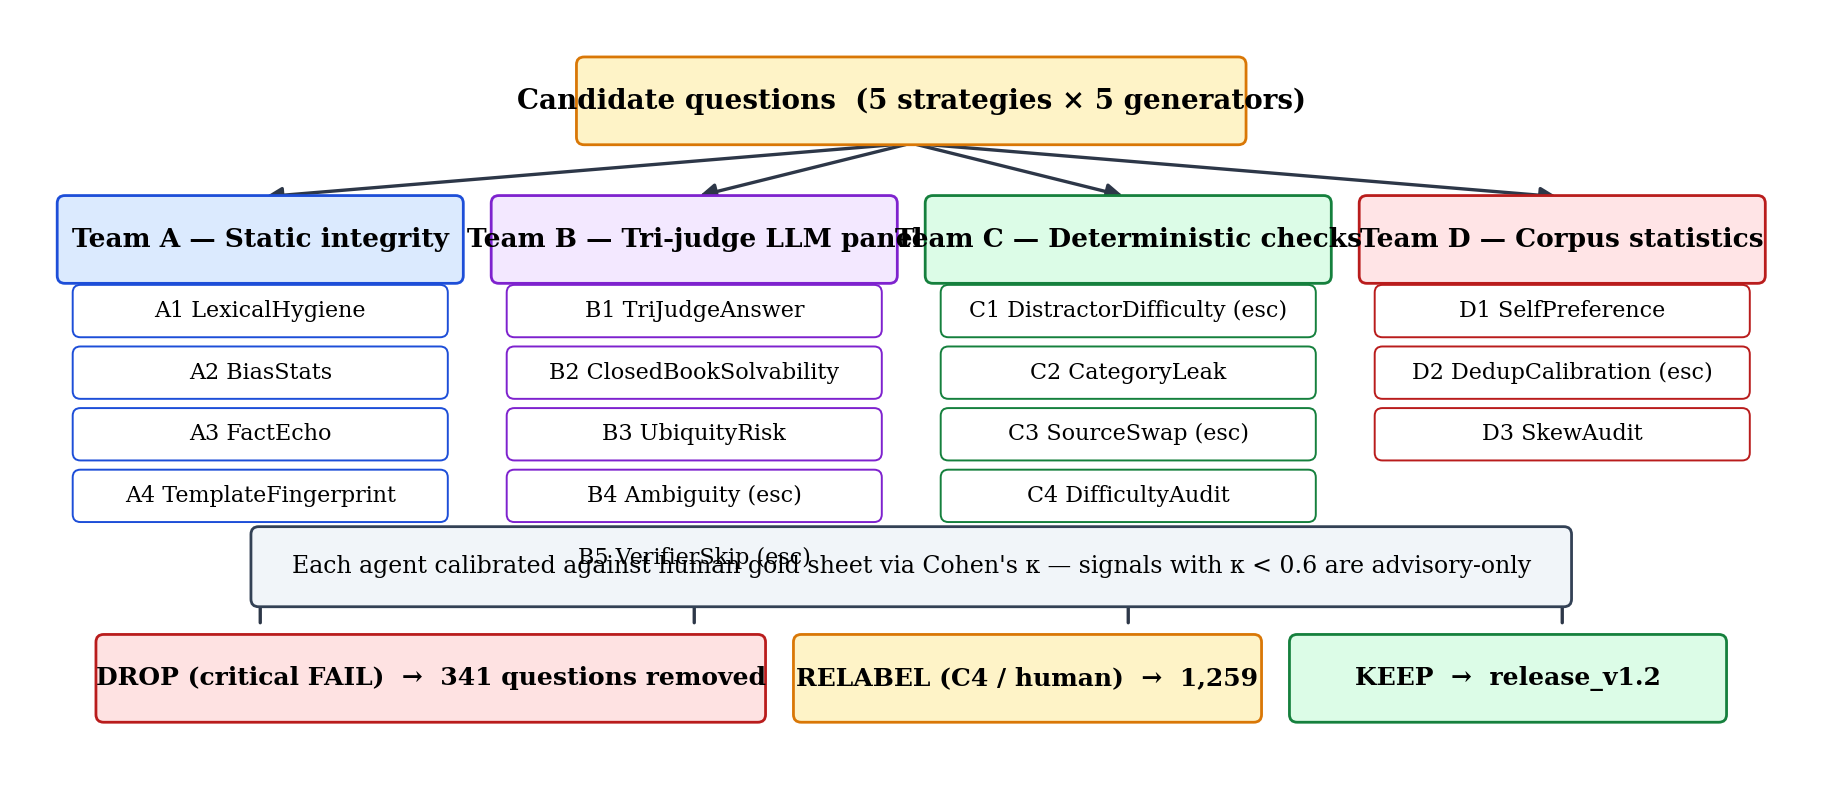
\includegraphics[width=0.95\linewidth]{figures/diagram_quality_assurance.png}
  \caption{Multi-agent audit architecture. Candidate questions are
    fanned out to four teams; each team independently emits per-question
    verdicts. Critical \textsc{fail} signals route the question to the
    drop pool; C4 difficulty disagreements route to relabel; otherwise
    the question is kept in \texttt{release\_v1.2}. Every agent is
    calibrated against the human gold sheet via Cohen's $\kappa$.}
  \label{fig:audit-app}
\end{figure}

\subsection{Atomic fact extraction pipeline}
\label{app:fact-extraction}

\begin{figure}[h]
  \centering
  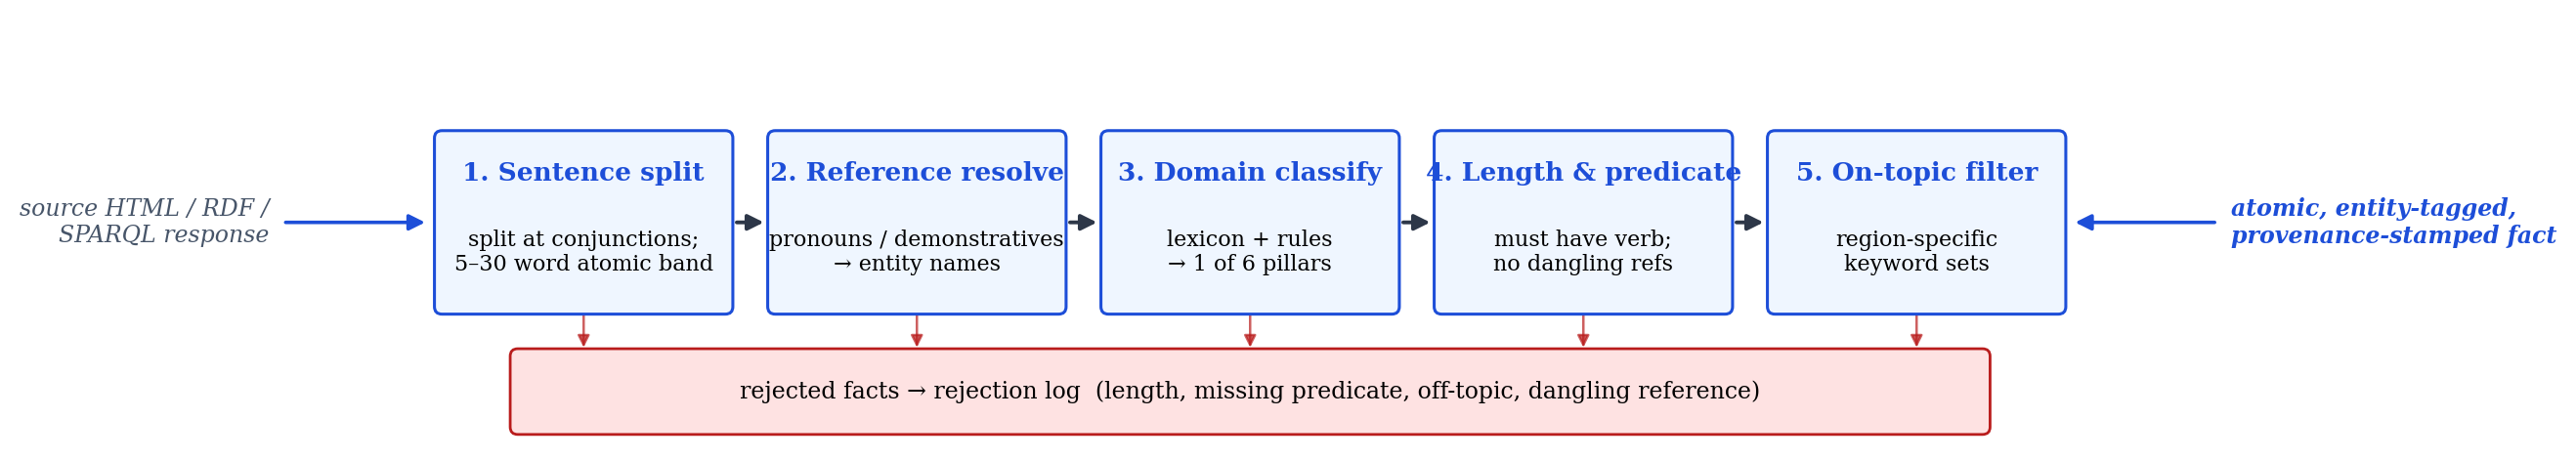
\includegraphics[width=0.85\linewidth]{figures/diagram_fact_processing.png}
  \caption{Atomic-fact extraction pipeline. Inputs are heterogeneous
    (HTML pages, RDF graphs, SPARQL responses, CSV dumps); outputs are
    uniform single-assertion sentences with entity tags, domain label,
    source URL and tier.}
  \label{fig:fact_processing}
\end{figure}

The atomic-fact extractor (\texttt{src/scrapers/\_fact\_processing.py})
applies five sequential filters to each candidate sentence:

\begin{enumerate}\itemsep -1pt
  \item \textbf{Sentence split.} NLTK Punkt tokeniser; further split at
    explicit conjunctions (``and'', ``but'', ``while'') when both clauses
    have an independent verb. Maximum atomic length 30~words; reject
    longer.
  \item \textbf{Reference resolution.} Pronouns and demonstratives are
    replaced with their entity referent from article context (paragraph-level
    coreference using a rule-based resolver tuned on Wikipedia
    leads). Sentences with unresolved \emph{it/this/that} are dropped.
  \item \textbf{Domain classification.} Lexicon-based + rule-based
    classifier maps each fact to one of the six domain pillars; ambiguous
    facts (no anchor term in any domain lexicon) are dropped.
  \item \textbf{Length and predicate validation.} Reject facts $<$5
    words, $>$50 words, missing a verb, or carrying dangling
    references / fragments. The 5--30 word band is the strict filter;
    the 31--50 band is kept with reduced confidence (910 facts).
  \item \textbf{On-topic filter.} Region-specific keyword sets prevent
    cross-contamination (e.g.\ Austrian content in a Bordeaux scraper).
    Fail $\Rightarrow$ drop.
\end{enumerate}

A 2026-04 audit found that 19 of an original 35 scrapers contained
hard-coded LLM-generated facts disguised as scraped data. The fix
required rebuilding all 19 against live sources; the lesson preserved
for future retargeting is that \emph{provenance auditing must run on
the scrapers themselves}, not only on the collected facts.

\subsection{Wikidata SPARQL: P17 vs P131*}
A common bug in early scrapers used the transitive administrative-parent
property (\texttt{P131*}) to bind questions to a country. This introduced
severe cross-region contamination, e.g.\ Austrian appellations appearing
in a Bordeaux scraper because the SPARQL graph traversal walked through
shared ancestor entities. Switching to the direct country relation
(\texttt{P17}) eliminated cross-country leakage at the cost of
$\sim$3\% lost coverage on borderline-region entities. The released
SPARQL templates use \texttt{P17} exclusively and we recommend the same
discipline for any pipeline retargeted to a domain with hierarchical
political subdivisions.

\subsection{Question-generation prompts}
The five strategies share a common JSON output schema enforced via
Pydantic with a 3-tier extraction fallback (markdown-fenced, raw JSON,
prefix-pattern). Per-strategy prompt summaries:

\begin{itemize}\itemsep -1pt
  \item \textbf{Fact-to-question:} "Given a single atomic wine fact,
    write a 4-option multiple-choice question whose unique correct
    answer is grounded in the fact. Paraphrase the fact; do not copy
    contiguous spans of $>$5 words. Distractors must be confusable
    same-category entities, not random alternatives."
  \item \textbf{Comparative:} given two related facts (matched on
    entity type, country/sub-domain), "ask which differs in the named
    attribute or what both share. Avoid iconic-vs-non-iconic pairings."
  \item \textbf{Scenario synthesis:} given a cluster of 3--5 facts,
    "write a brief domain-appropriate professional scenario (sommelier
    service / winemaker decision / viticulturist call /
    business/regulatory choice) with a unique correct answer that
    requires \emph{all} the cluster facts to derive."
  \item \textbf{Distractor mining:} given a fact + 3 confusable
    entities, "write a question whose 3 wrong options are these
    entities, ranked by ascending plausibility."
  \item \textbf{Template:} 45 deterministic parameter substitution
    templates; no LLM call. A subset is paraphrased post-hoc by Gemini
    Pro to defeat the A4 stylometric fingerprint detector.
\end{itemize}

Full prompt texts are in
\texttt{src/generators/\_prompts.py}.

\subsection{Closed-book gate specification}
The closed-book pre-screen (\texttt{src/generators/\_closed\_book\_gate.py})
runs a per-difficulty model:

\begin{itemize}\itemsep -1pt
  \item L1: Claude Haiku 4.5 reads the question with no source fact.
    Correct answer~$\Rightarrow$ tag \texttt{closed\_book\_solvable}.
  \item L2: Claude Sonnet 4.6 same protocol.
  \item L3: Claude Opus 4.7 same protocol; the corpus quota cap fires
    here.
  \item L4: gate is skipped by protocol; expert items are expected to
    be answerable only with the source fact.
\end{itemize}

The gate's role in generation is to enforce a corpus-level cap on
closed-book-solvable items; early pilots used a 25\% cap, but it was
\textbf{raised to 50\%} after the gold-sheet calibration revealed that
the LLM panel over-attributes closed-book solvability relative to
humans (Section~\ref{sec:gold}), so the higher cap retains the items
that are in fact discriminating in evaluation. The audit's B2 agent
later re-runs the check at corpus scale on a tri-judge panel.
Failures are not dropped; they are reserved into the closed-book
slice and used for the analytic partition in
Section~\ref{sec:eval-cb}.

\subsection{Audit agent specifications}
\label{app:audit-agents}
Each agent is a versioned Python module under \texttt{src/qa/agents/}.
Agents emit
\texttt{(question\_id, agent\_id, version, severity, payload\_json)}
tuples to the \texttt{audit\_findings} table; \texttt{severity} is one
of \{\textsc{pass}, \textsc{warn}, \textsc{fail}\}. Versioning is
strict: the (\texttt{run\_id}, \texttt{question\_id}, \texttt{agent\_id},
\texttt{version}) tuple is unique, so re-running an agent at a new
version produces additive findings rather than overwriting. We document
each agent's threshold and gold-sheet $\kappa$ here.

\begin{table}[h]
  \centering
  \footnotesize
  \caption{Audit-agent thresholds and gold-sheet calibration.}
  \label{tab:agent-thresholds}
  \begin{tabular}{lllr}
    \toprule
    Agent & Signal & Threshold & $\kappa$ vs.\ gold \\
    \midrule
    A1 LexicalHygiene      & vague/marketing regex hits & $\geq$1 hit $\Rightarrow$ \textsc{warn}; $\geq$3 $\Rightarrow$ \textsc{fail} & 0.71 \\
    A2 BiasStats           & $\chi^2$ position; M--W length & $p<0.01 \Rightarrow$ \textsc{fail} & 0.65 \\
    A3 FactEcho            & LCS / fact length          & $\geq$0.45 $\Rightarrow$ \textsc{warn}; $\geq$0.65 $\Rightarrow$ \textsc{fail} & 0.83 \\
    A4 TemplateFingerprint & POS-bigram logreg held-out AUC & $>0.84$ corpus-level $\Rightarrow$ \textsc{warn} & 0.62 \\
    B1 TriJudgeAnswer      & majority disagrees with key & 2/3 disagree $\Rightarrow$ \textsc{fail} & 0.78 \\
    B2 ClosedBookSolv.     & majority solves no-source & 2/3 solve $\Rightarrow$ \textsc{warn}; 3/3 $\Rightarrow$ \textsc{fail} & \textbf{0.007} \\
    C2 CategoryLeak        & wine-type mismatch in distractors & any $\Rightarrow$ \textsc{fail} & 0.91 \\
    C4 DifficultyAudit     & $|\Delta|$ assigned vs.\ rated & $\geq$1 \textsc{warn}; $\geq$2 \textsc{fail} & 0.74 \\
    B3 UbiquityRisk        & ubiquitous-grape stem $\times$ region answer & both $\Rightarrow$ \textsc{warn} & 0.69 \\
    \bottomrule
  \end{tabular}
\end{table}

The B2 row is the calibration finding discussed in
Section~\ref{sec:gold}: the LLM panel and the human reviewer disagree
on what counts as ``world-knowledge solvable'', because frontier LLMs
have absorbed substantial wine knowledge during pre-training. We retain
the agent as a measurement of the LLM panel's prior, and report the
contextual / closed-book partition (Section~\ref{sec:eval-cb}) that
turns the disagreement into a useful diagnostic.

\paragraph{Release-cycle audit findings.}
Table~\ref{tab:audit_results} summarises the verdicts produced when
the 9-agent audit was applied to \texttt{release\_v1.1} (3{,}670
candidate questions); these are the numbers cited in
Section~\ref{sec:audit-results}.

\begin{table}[h]
  \centering
  \caption{Audit findings on \texttt{release\_v1.1} and the resulting
    drop / re-label policy.}
  \label{tab:audit_results}
  \footnotesize
  \begin{tabular}{lrl}
    \toprule
    Audit signal & Triggered FAIL & Action \\
    \midrule
    A1 LexicalHygiene (vague phrasing)               & 60   & drop \\
    A3 FactEcho (verbatim copy)                      & 63   & drop \\
    B1 TriJudgeAnswer (wrong answer key)             & 47   & drop \\
    C2 CategoryLeak (wine-category leak)             & 9    & drop \\
    B3 UbiquityRisk (grape $\times$ region ambiguity)& 183  & drop \\
    \midrule
    Distinct dropped (with overlap)                  & \textbf{341} & \\
    \midrule
    C4 DifficultyAudit (relabel from 1{,}252 LLM hits + 7 human)
                                                     & 1{,}259 & re-label \\
    B2 ClosedBookSolvability (kept w/ disclosure)     & 1{,}601 & disclose \\
    \bottomrule
  \end{tabular}
\end{table}

\paragraph{Difficulty distribution before and after C4 re-label.}
Table~\ref{tab:difficulty-shift} shows the corpus-level effect of the
C4 difficulty re-label, which shifted the corpus from 14\% L3+L4 items
to 51\% L3+L4.

\begin{table}[h]
  \centering
  \caption{Difficulty distribution before and after C4 re-label.}
  \label{tab:difficulty-shift}
  \footnotesize
  \begin{tabular}{lrrr}
    \toprule
    & Generator-assigned & Post-relabel & $\Delta$ \\
    \midrule
    L1 (entry)        & 1{,}261 (38\%) & 694   (21\%) & $-567$ \\
    L2 (intermediate) & 1{,}559 (47\%) & 894   (27\%) & $-665$ \\
    L3 (advanced)     &   218 ( 7\%) & 678   (21\%) & $+460$ \\
    L4 (expert)       &   291 ( 9\%) & 1{,}001 (31\%) & $+710$ \\
    \bottomrule
  \end{tabular}
\end{table}
